% !TeX spellcheck = en_US

\chapter{Concept and Architecture}\label{chap:conarch}
In this chapter, the concept and the architecture of the framework which can satisfy the requirements will be explained and substantiated.
The chosen solution will resolve data download commands and package installation commands.
%A user will have an opportunity to chose the method of the encapsulation, the "sets of packages" or "one node for one package" which were described in section~\ref{subs:encaps}.
Solutions to some additional problems will be presented. 
\section{Concept}
In this section, the main concept of this work are described.
The general structure of the framework is visualized in Figure~\ref{fig:gen}. 
In section~\ref{subs:analyse}, it will be explained how to determine the Node Templates which use the given artifact.
Then language modules, package manager modules and download tool modules functionality will be presented.
In section~\ref{subs:repres}, it will be expressed how to create a new node for a TOSCA topology. 
After that, some methods to determine the architecture of the final platform will be presented.
In addition, it will be described, how the results can be validated.
% !TeX spellcheck = en_US

\begin{figure}
	\centering
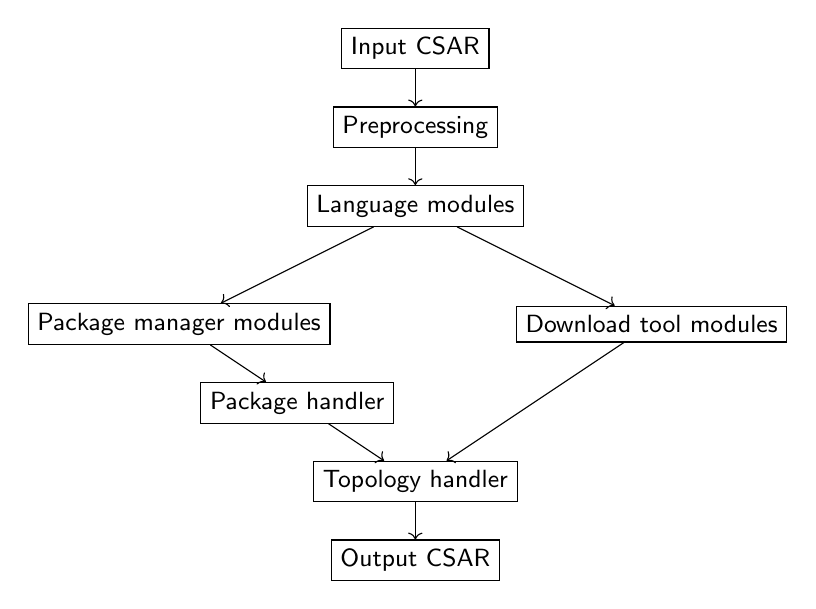
\begin{tikzpicture}
\node[draw] (in) at (0,1.5) {Input CSAR};
\node[draw] (pp) at (0,+0.5) {Preprocessing};
\node[draw] (lm) at (0,-0.5) {Language modules};
\node[draw] (pmm) at (-3,-2) {Package manager modules};
\node[draw] (dtm) at (+3,-2) {Download tool modules};
\node[draw] (ph) at (-1.5,-3) {Package handler};
\node[draw] (th) at (0,-4) {Topology handler};
\node[draw] (out) at (0,-5) {Output CSAR};
\draw [->] (in) -- (pp);
\draw [->] (pp) -- (lm);
\draw [->] (lm) -- (pmm);
\draw [->] (lm) -- (dtm);
\draw [->] (pmm) -- (ph);
\draw [->] (dtm) -- (th);
\draw [->] (ph) -- (th);
\draw [->] (th) -- (out);
\end{tikzpicture} 
\caption{The general description of the software's work flow} 	\label{fig:gen}
\end{figure}

\subsection{Analysis of a TOSCA-Topology}\label{subs:analyse}
To update the \gls{tosca} topology properly, it is necessary to add references from the nodes where external references were to the newly created nodes which resolve the external references. 
According to TOSCA standard, references between Node Templates can only be created in the same Service Template.  
That means that each Node Template which uses artifacts with external references must be found.
Furthermore, Service Template where these Node Templates are instantiated must be determined to create there a Node Template for the new nodes and reference them to the Node Templates with external references.
The pointers to artifacts are contained by Artifact Templates which are used by Node Type Implementations.
By composing all the information the simple references chain can be built:\\
$Artifact$ $\rightarrow$ $Artifact$~$Template$ $\rightarrow$ $Node$~$Type$~$Implementation$ $\rightarrow$ $Node$~$Type$ $\rightarrow$ $Node$~$Template$ $\rightarrow$ $Service$~$Template$\\
Now consider the references in more detail. 
\begin{itemize}
	\item $Artifact$ $\rightarrow$ $Artifact$ $Template$\\
	An Artifact can be referenced by several Artifact Templates. (Despite the fact that this is a bad practice.)
	\item  $Artifact$ $Template$ $\rightarrow$ $Node$ $Type$ $Implementation$ \\
	The same way an Artifact Template can be used by several Node Type Implementations.
	\item $Node$ $Type$ $Implementation$ $\rightarrow$ $Node$ $Type$ \\
	A Node Type Implementation can describe an implementation of only one Node Type.
	\item  $Node$ $Type$ $\rightarrow$ $Node$ $Template$\\
	Each Node Type can have any number of Node Templates.
	\item  $Node$ $Template$ $\rightarrow$ $Service$ $Template$\\
	But each Node Template is instantiated only once.
\end{itemize}
This structure can be described as a tree with an Artifact as a root, and Service Templates as leaves and will be called the internal dependencies tree.
The example is provided by Figure~\ref{fig:script_serv}.\\
%Of course it is possible to move in opposite direction, starting from a Node and moving toward scripts, but this method brings additional complexity. 
There is an additional problem in the reference between a Node Type and a Node Type Implementation.
A Node Type can have several implementations, but which one will be used is determined only during the deployment. 
The chosen solution to this problem is to use each Node Type Implementation in the hope, that they will not conflict.\\
%The method presented above can uniquely determine Node Templates and Service Template for a given script.
%Of course it is not guaranteed that found Node Type Implementation will be used during deployment, but we can't do anything with this. 
The following steps to build the internal dependencies tree can be executed during the preprocessing.
\begin{itemize}
	\item Find all Artifact Templates to build references from Artifacts to Artifact Templates.
	\item Find all Node Type Implementations. 
		Since they contain references both to the Node Type and to the Artifact Templates, so the dependency from Artifact to Node Types can be built.
	\item Find all Service Templates and all contained Node Templates they contain. 
		Each Node Template contains a reference to Node Type what is useful for building a dependency from Artifact to Node Template.
\end{itemize} 
In this way the required internal dependencies tree with references $Artifact$ $\rightarrow$ $Node$~$Template$ and $Artifact$ $\rightarrow$ $Service$~$Template$ can be built.
% !TeX spellcheck = en_US
\usetikzlibrary{calc,arrows.meta,positioning}
\tikzset{
    every node/.style={font=\sffamily\small},
    main node/.style={shape=rectangle, rounded corners,
    	draw, align=center,
    	top color=white, bottom color=blue!20}
}

\begin{figure}
	\centering
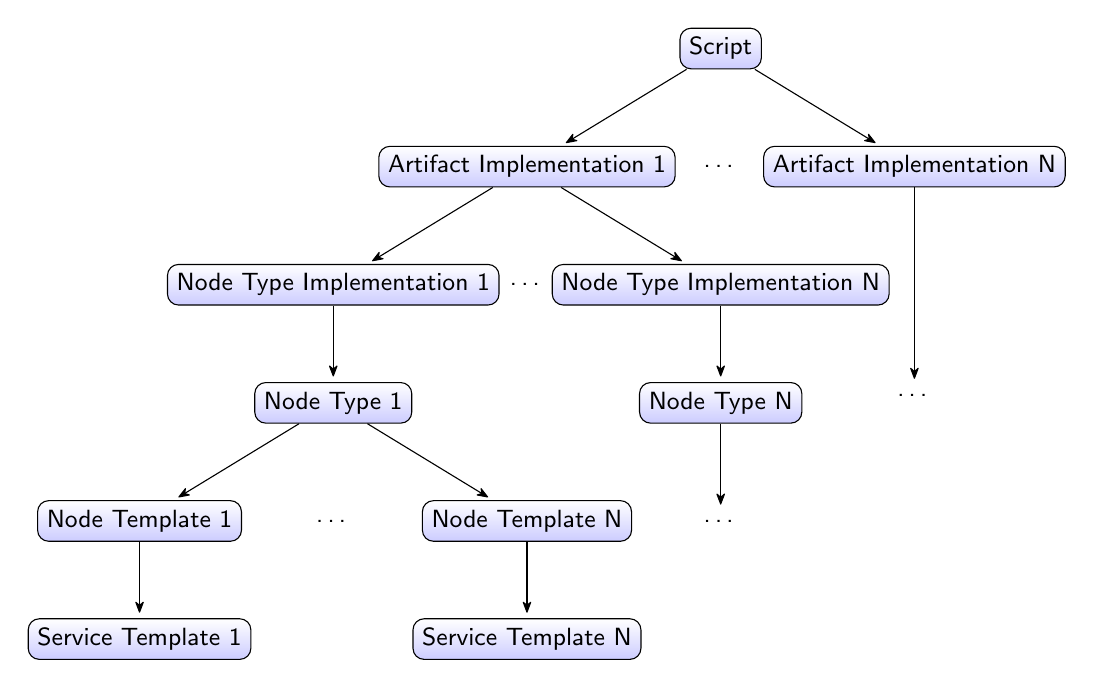
\begin{tikzpicture}[sibling distance=14em,->,>={Stealth[round,sep]},shorten >=1pt,auto,node distance=25mm]
    \node[main node] (1) {Script}
    child { node[main node](3) {Artifact Implementation 1} 
    	child { node[main node] (6) {Node Type Implementation 1} 
    			child { node[main node] (8) {Node Type 1} 
    				child { node[main node]  (11) {Node Template 1} 
    					child { node[main node] (13) {Service Template 1}}  
    				}
    				child { node[main node]  (12) {Node Template N} 
    					child { node[main node] (14) {Service Template N}}
    				}
    			}
    	}
    	child { node[main node] (7) {Node Type Implementation N} 
    		child { node[main node] (9) {Node Type N} 
    			child { node  (10) {\ldots} }
    		}
    	}
    }
    child { node[main node] (4) {Artifact Implementation N}  
    child { node (5) [below =of 4]{\ldots}}
	};

    \node at ($(3)!.5!(4)$) {\ldots};
    \node at ($(6)!.5!(7)$) {\ldots};
    \node at ($(11)!.5!(12)$) {\ldots};
    
\end{tikzpicture} 
\caption{Example tree describing how to find Service Templates and Node Templates for a given script} 	\label{fig:script_serv}
\end{figure}

\subsection{Search for Artifacts}
Since external references are stored in artifacts, we need to find all of them in order to identify the references.
The first simple solution is to analyze the structure of a TOSCA application and identify all artifacts used.
But this method brings an possibility to miss artifacts because some of them can be called from other artifacts.
This case is presented by Figure~\ref{fig:artart}.
In this example Implementation Artifact Engine calls the "Artifact 1" which calls the "Artifact 2".
The "Artifact 2" isn't called by Implementation Artifact Engine directly and therefore will not be considered by the method described above.
The found solution is to analyze all files presented in an input CSAR and resolve external references in all of them.
One needs to define methods to identify scripts for each supported configuration management tool.
% !TeX spellcheck = en_US

% We need layers to draw the block diagram
\usetikzlibrary{calc,positioning}
\usetikzlibrary{arrows.meta}

% Define a few styles and constants
\tikzstyle{entry}=[draw, minimum height=2em, align=center]
\tikzstyle{mytext}=[align=center]
\tikzstyle{frame} = [entry, text width=28em, fill=white,minimum height=10em, rounded corners]
\tikzstyle{engine} = [entry, text width=7em, fill=white,minimum height=4em, rounded corners, left color=green!15!white, right color=green!20!white,shading angle=135, anchor=north]
\tikzstyle{store} = [entry, text width=16em, fill=white,minimum height=6em, rounded corners, left color=blue!15!white, right color=blue!20!white,shading angle=135, anchor=north]
\tikzstyle{art} = [entry, text width=5em, fill=white,minimum height=3em, rounded corners, left color=red!15!white, right color=red!20!white,shading angle=135, anchor=north]
\def\blockdist{2.3}
\def\edgedist{2.5}

\begin{figure}
	\centering
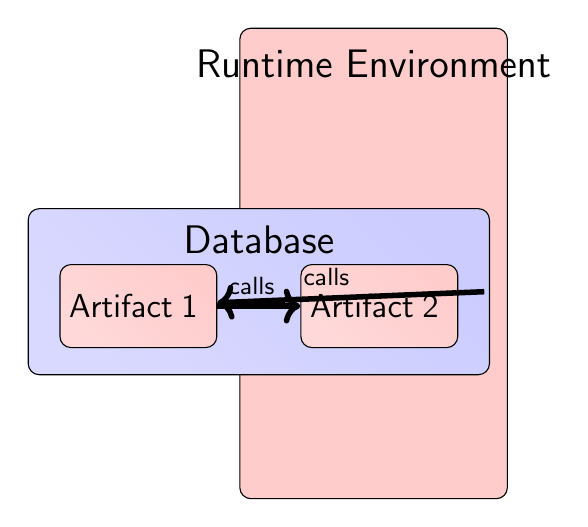
\begin{tikzpicture}
\node (frame) [frame, label={[shift={(+0ex,-5ex)}]north:{\Large Runtime Environment}}] {};

\node (engine) [xshift=+5em, yshift=+1em] at (frame.west) [engine] {\large Management plan};
\node (storage) [xshift=-9em, yshift=+2em] at (frame.east) [store,label={[yshift=-2em]north:{\Large Database}} ] {};

\node (art1) [xshift=+4em, yshift=+1em] at (storage.west) [art] {\large Artifact 1};
\node (art2) [xshift=-4em, yshift=+1em] at (storage.east) [art] {\large Artifact 2};

\draw [->,scale=5,line width=2pt] (engine.east) --node [text width=2.5cm,midway,above ] {~~~~~~calls} (art1);
\draw [->,scale=5,line width=2pt] (art1.east) --node [text width=2.5cm,midway,above] {~~~~~~~~calls} (art2);

\end{tikzpicture} 
\caption{Bad artifacts call sequence} 	\label{fig:artart}
\end{figure}

\subsection{Modules and Extensibility}
The framework should handle different languages, each of which can support various package managers and data download tools.
It was decided to develop a modular system, where modules handle the above listed elements.
The chosen solution is to create the software which will contain and support language modules handling configuration management tools.
Each language module itself will contain and support package managers modules and download tool modules which handle package managers and data download tools respectively.
A language module should filter files not belonging to the language and the accepted files will be transmitted to the supported modules.
A package manager module resolves an external reference and transmits the package name from this reference to a package handler described in section~\ref{subs:archph}.
A data download module identifies download commands, removes them, downloads the data and calls a topology handler defined in section~\ref{subs:archtop}. 
This principle can be illustrated by Figure~\ref{fig:lang_pm}.
Ease of adding of new modules to the framework will prove the correctness of this system.\\
It is impossible to identify all types of external references, even when only one language and one package manager are used.
An example can be found in listing~\ref{alg:unreadable}.
Since this work is aimed at creating the easily expanded and supplemented tool, then only basic usage of package managers will be considered initially.\\
At the beginning the most popular combination must be developed: the $bash$ language with the $apt-get$ package manager.
This simple and powerful tool allows to install, delete or update the set of packages in one line of code.
A line-by-line parser which analyses scripts and finds the installation commands can parse such commands must be developed.
After the modules for this combination will be implemented and validated, new language and package manager modules can be added.
\begin{Listing} 
	\caption{Unreadable bash script}
	\label{alg:unreadable}
	\begin{lstlisting}
	#!/bin/bash
	set  line = abcdefgijklmnoprst
	# The "line" contains a part of the alphabet
	set  word1 = ${line:0:1}${line:14:1}${line:17:1} 
	# The 1th, 15th and 18th letters of the "line" variable are stored into the "word1".
	# "word1" will contain the "apt" string 
	set  word2 = ${line:6:1}${line:4:1}${line:17:1}
	# The 7th, 5th and 18th letters of the "line" variable are stored into the "word2".
	# "word2" will contain the "get" string 
	$word1-$word2 install package
	# This is the "apt-get install package" command,
	#		 but to determine that a good interpreter is needed.
	\end{lstlisting}
\end{Listing}
% !TeX spellcheck = en_US

% We need layers to draw the block diagram
\usetikzlibrary{calc,positioning}

% Define a few styles and constants
\tikzstyle{entry}=[draw, fill=green!20, minimum height=2.5em]
\tikzstyle{ann} = [above, text width=5em]
\tikzstyle{framework} = [entry, text width=35em, fill=red!20, 
minimum height=18em, rounded corners]
\tikzstyle{lang} = [entry, text width=9em, fill=blue!20, 
minimum height=15em, rounded corners]
\def\blockdist{2.3}
\def\edgedist{2.5}

\begin{figure}
	\centering
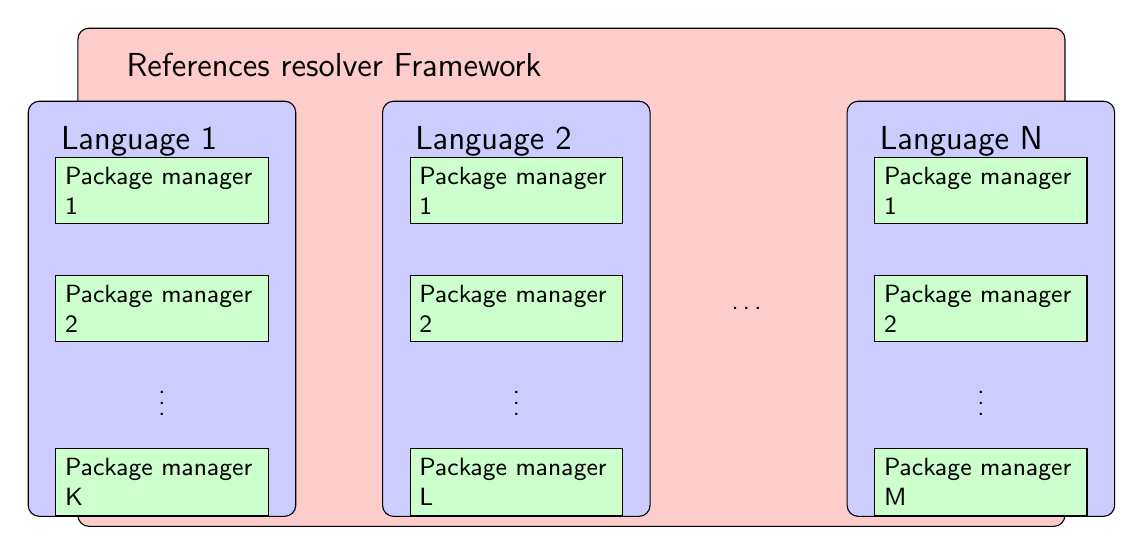
\begin{tikzpicture}
\node (rr) [framework] {};
\node [xshift=+5mm, yshift=-2mm, below right] at (rr.north west) {\large References resolver Framework };


\node (lang1) at ([xshift=-52mm,yshift=-4mm]rr) [lang] {};
\node [xshift=+3mm, yshift=-2mm, below right] at (lang1.north west) {\large Language 1 };
\node (lang2) at ([xshift=-7mm,yshift=-4mm]rr) [lang] {};
\node [xshift=+3mm, yshift=-2mm, below right] at (lang2.north west) {\large Language 2 };
\node (langn) at ([xshift=+52mm,yshift=-4mm]rr) [lang] {};
\node [xshift=+3mm, yshift=-2mm, below right] at (langn.north west) {\large Language N };
\node at ($(lang2)!.5!(langn)$) {\ldots};

\node (l1pm1) at ([yshift=+15mm]lang1) [entry] {Package manager 1};
\node (l1pm2) at ([yshift=0mm]lang1) [entry] {Package manager 2};
\node (l1pmn) at ([yshift=-22mm]lang1) [entry] {Package manager K};
\node at ($(l1pm2)!.5!(l1pmn)$) {\vdots};

\node (l2pm1) at ([yshift=+15mm]lang2) [entry] {Package manager 1};
\node (l2pm2) at ([yshift=0mm]lang2) [entry] {Package manager 2};
\node (l2pmn) at ([yshift=-22mm]lang2) [entry] {Package manager L};
\node at ($(l2pm2)!.5!(l2pmn)$) {\vdots};

\node (lnpm1) at ([yshift=+15mm]langn) [entry] {Package manager 1};
\node (lnpm2) at ([yshift=0mm]langn) [entry] {Package manager 2};
\node (lnpmn) at ([yshift=-22mm]langn) [entry] {Package manager M};
\node at ($(lnpm2)!.5!(lnpmn)$) {\vdots};


\end{tikzpicture} 
\caption{Example scheme representing several languages and package managers} 	\label{fig:lang_pm}
\end{figure}
\subsection*{Encapsulation of CSARs with extarnal Packages}\label{subs:encaps}
Here will be define some methods of encapsulation of a CSAR containing external packages.

%It will be defined two methods  which install external packages during the deployment.
%The encapsulation must be achieved through the download of external packages and generation of a new TOSCA node for each of them. 
%But it can be interesting to analyze other techniques to encapsulate a CSAR. 
At first, one will describe the $generate$ $custom$ $repositories$ and $generate$ $shared$ $repositories$ methods not representing packages in a TOSCA topology and then the $one$ $node$ $for$ $one$ $package$ and $sets$ $of$ $packages$ methods mirroring packages into the topology.
\subsubsection*{Generate Custom Repositories}
It's possible to download all necessary packages and create one's own custom package repository for each operating system used in the application. 
Then one must rework any package installation commands or exchange system preferences to setup an access to the custom repository.
This method introduces minimal changes in a TOSCA structure.
The main problem is the creation of the custom repositories. 
When a TOSCA application consists of many small devices with limited capabilities it can be difficult to start many big custom repositories.
\subsubsection*{Generate Shared Repository}
Another opportunity is to create a single repository for all devices in a TOSCA application.
It can be difficult to choose the right location for such a server, but since an application represents the connected system this step can redistribute the load to a more powerful device.
It is difficult to estimate the changes which will occur in a TOSCA topology while applying such a method.
\subsubsection*{One Node for One Package}
%This method was suggested by the \gls{uniiaas}. 
A new TOSCA node will be created for each downloaded package. 
All dependencies between packages will be mirrored to a TOSCA topology.
This is a very visual method, facilitating the understanding of a TOSCA application and dependencies between packages.
\subsubsection*{Sets of Packages} \label{mode:setsofpkg}
A set of depended packages from a dependencies tree related to an external reference can be combined and represented in a TOSCA topology as a single node.
An installation of such a node will lead to the installation of all needed packages.
This way a small size of a TOSCA application's structure will be achieved.
It will be impossible to trace dependencies (since many packages are represented by one node), but it can help to avoid a difficult structure which consists of hundreds of nodes. 

\subsection{Encapsulation of CSARs with extarnal files}
%At the startup of the software, a user will be able to choose modes of operation.
%It was developed the concepts for two modes for external references presented by package installations and two modes for external references presented by file downloads.
%The default mode for package processing is the "one node for one package" mode. 
%In this mode, a new TOSCA node will be created for each used package from a packages database and dependencies between packages from the database will be mirrored to a TOSCA topology.
%Besides the default mode of operation, the "sets of packages" mode described in section~\ref{mode:setsofpkg} will be developed to provide possibility to generate relatively small encapsulated applications.
%This mode will be called the single node mode.
%To create the sets properly, the language module must combine the information about all packages needed for an artifact and then create a single TOSCA node for all of them.\\
It was developed two modes to process external files.
The first possibility is to create a new TOSCA node which contains a deployment artifact presenting the downloaded file and an implementation artifact which will try to put the file into the right place.
But one can't be sure that this file will be available for other nodes.
In the second mode, downloaded files must be integrated into the node which contain the download command.
The download command can be exchanged by a file move command to put the file in the right position.

\subsection{Representing Downloaded Packages in a TOSCA-Topology} \label{subs:repres}
Downloaded data must be represented in the structure of a Cloud Application. 
A package node denotes the defined and instantiated element of the \gls{tosca} topology, the purpose of which is to install packages.
And a file node denotes the defined and instantiated element of the \gls{tosca} topology, the purpose of which is to store files.
The addition of new package and file nodes to the TOSCA topology can be divided into several steps.
\begin{itemize}
	\item One must add definitions for common elements like Artifact Types or Relationship Types. 
		This can be done once.
	\item The package node common definition will be represented by a Node Type. 
		It must contain the $install$ operation, which represents the capability to install the node.
		For the package nodes that will cause the installation of the package, and for the file nodes it is the file move operation.
		%There will be described that this node must be installed.
	\item Artifacts (downloaded data and installation scripts) will be referenced by Artifact Templates.
	\item A Node Type Implementation will combine the Artifact Templates to implement the $install$ operation.
	\item A Node Template will instantiate a node in the corresponding Service Templates.
		To determine the corresponding Service Template the autor will use the preprocessing described in the section~\ref{subs:analyse}.
	\item A Reference Template will provide topology information allowing the observer (a user or a runtime environment) to determine which nodes the package must be installed for.
		References will be created from the Node Template which needs the created node to the Node Template of the created nodes.
\end{itemize}
After an execution of these steps, a definition of a node will be finished and it can be used.

\subsection{Determining Architecture of the Final Platform} \label{finplatf}
To download the right instance of a package one must define its architecture.
It can be difficult to predict the architecture of the device where packages will be installed.
Unfortunately, it is impossible to analyze the structure of any CSAR and determine the architecture of the device which node will be deployed on.
There are many pitfalls here.\\
A single Service Template can use several physical devices with different architectures.
Many Node Types and Node Templates instantiated on different platforms can refer to the same Implementation Artifact.
This way one simple Implementation Artifact with a bash script containing the "$apt$-$get$ $install$ $python$" command can be deployed on different devices within one Service Template (for example with the arm, amd64 and i386 architectures) and will result in the download and installation of three different packages. 
For an end user, the ability to use such a simple command is a huge advantage, but for the framework, it can greatly complicate the analysis.
The following methods of architecture selection were designed.
\begin{itemize}
	\item $Deployment$ $environment$ $analysis$\\
	The script can analyze the system where it was started (for example using the "$uname$~$-a$" command) and depending on the result, it will install the package corresponding to the system's architecture.
	\item $Unified$ $architecture$\\
	The architecture will be defined by the user for the whole CSAR.
	\item $Artifact$ $specific$ $architecture$\\
	The architecture will be defined for each artifact separately.
\end{itemize}
%\subsubsection*{Analysis of methods}
The $deployment$ $environment$ $analysis$, which at first sight seems to be the most reliable solution, brings many additional problems.
Packages for different platforms can differ not only by architecture but also by the version and the list of dependencies.
As a consequence, chaos may occur while  mirroring these different packages with different versions to the \gls{tosca} topology.
The only found robust solution is to create a set of archives for each installed package. Using this method, data for one architecture are stored into one archive.
Such archives will contain the entire dependency tree for the given package.
But this approach contradicts one of the main ideas of this work: the dependencies trees should be mapped to the topology.\\
The $artifact$ $specific$ $architecture$ method carries an additional complexity to the user of the framework.
It will make a user to analyze each artifact and decide which architecture it will be executed on. 
This can be complicated by the fact that the same artifact can be executed on different architectures.\\
The method of the $unified$ $architecture$ was chosen as the simplest and easiest to implement.
If it will be necessary, this method can easily be expanded to the $artifact$ $specific$ $architectures$ method (by removing the user input at start, and choosing an architecture for each artifact separately) or to $deployment$ $environment$ $analysis$ (by downloading packages for all available architectures and adding the architecture determining algorithm to the installation scripts).

%\subsection{Extensibility}
%The framework should handle different languages, each of them can support various package managers.
%An language module should filter files not belonging to the language, accepted files will be processed 
%This principle can be illustrated by a Figure \ref{fig:lang_pm}.
%% !TeX spellcheck = en_US

% We need layers to draw the block diagram
\usetikzlibrary{calc,positioning}

% Define a few styles and constants
\tikzstyle{entry}=[draw, fill=green!20, minimum height=2.5em]
\tikzstyle{ann} = [above, text width=5em]
\tikzstyle{framework} = [entry, text width=35em, fill=red!20, 
minimum height=18em, rounded corners]
\tikzstyle{lang} = [entry, text width=9em, fill=blue!20, 
minimum height=15em, rounded corners]
\def\blockdist{2.3}
\def\edgedist{2.5}

\begin{figure}
	\centering
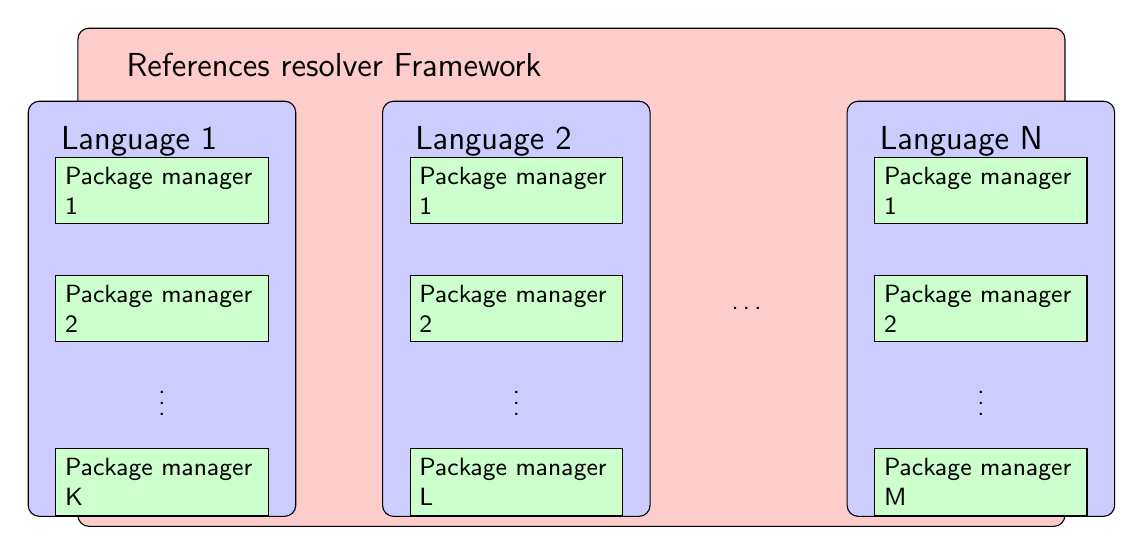
\begin{tikzpicture}
\node (rr) [framework] {};
\node [xshift=+5mm, yshift=-2mm, below right] at (rr.north west) {\large References resolver Framework };


\node (lang1) at ([xshift=-52mm,yshift=-4mm]rr) [lang] {};
\node [xshift=+3mm, yshift=-2mm, below right] at (lang1.north west) {\large Language 1 };
\node (lang2) at ([xshift=-7mm,yshift=-4mm]rr) [lang] {};
\node [xshift=+3mm, yshift=-2mm, below right] at (lang2.north west) {\large Language 2 };
\node (langn) at ([xshift=+52mm,yshift=-4mm]rr) [lang] {};
\node [xshift=+3mm, yshift=-2mm, below right] at (langn.north west) {\large Language N };
\node at ($(lang2)!.5!(langn)$) {\ldots};

\node (l1pm1) at ([yshift=+15mm]lang1) [entry] {Package manager 1};
\node (l1pm2) at ([yshift=0mm]lang1) [entry] {Package manager 2};
\node (l1pmn) at ([yshift=-22mm]lang1) [entry] {Package manager K};
\node at ($(l1pm2)!.5!(l1pmn)$) {\vdots};

\node (l2pm1) at ([yshift=+15mm]lang2) [entry] {Package manager 1};
\node (l2pm2) at ([yshift=0mm]lang2) [entry] {Package manager 2};
\node (l2pmn) at ([yshift=-22mm]lang2) [entry] {Package manager L};
\node at ($(l2pm2)!.5!(l2pmn)$) {\vdots};

\node (lnpm1) at ([yshift=+15mm]langn) [entry] {Package manager 1};
\node (lnpm2) at ([yshift=0mm]langn) [entry] {Package manager 2};
\node (lnpmn) at ([yshift=-22mm]langn) [entry] {Package manager M};
\node at ($(lnpm2)!.5!(lnpmn)$) {\vdots};


\end{tikzpicture} 
\caption{Example scheme representing several languages and package managers} 	\label{fig:lang_pm}
\end{figure}

\subsection{Validation}
Checking the output of the framework is an important stage in the development of the program.
It is necessary to verify both the internal correctness of the output \gls{csar} and the possibility to deploy generated package nodes.
The validity of internal dependencies can be checked by $Winery$ tool from OpenTOSCA.
This tool allows create and edit CSAR archives and is also great for visualizing the results.
Checking the deployment of the generated nodes can be done manually by entering commands which start the artifact's execution.


\section{Architecture}\label{sec:arch}
This section will present the architecture of the framework and the detailed description of its elements.
The main elements are a \boldmath $CSAR$ $handler$, a $references$ $resolver$, $language$ $modules$, $package$ $manager$ $modules$, a $package$ $handler$, and a $topology$ $handler$. \unboldmath

\subsection{CSAR handler} \label{subs:casr_h}
The CSAR handler provides an access to a \gls{csar} and maintains its consistency. 
It defines the method to add new files handling the metadata, \mbox{archiving/unarchiving}, and choosing the final platform architecture. \\
The input CSAR is initially archived and must be decompressed first in order to handle the content.
When all external references will be resolved, the content will be archived to an output CSAR.
A new name-value pair must be added to the metadata for each new file integrated into the CSAR during processing. 
The name represents the full path to the file and the value contains the type of the file. 
This type will be used by a runtime environment to chose the right behavior. %\\ %\\
As it was mentioned in section~\ref{finplatf}, an architecture of the final platform will be chosen for the entirely CSAR.
A command line interface must be provided for a user, to allow him to chose the architecture. 
The chosen architecture must be saved to the CSAR for the case of future processing by the framework to avoid the collisions between architectures of packages.

\subsection{References Resolver} \label{subs:RR}
References Resolver is the main element, whose execution is divided into three stages: $preprocessing$, $processing$, $finishing$. \\
During the $preprocessing$ stage, the CSAR will be unarchived, common files added, and internal dependencies trees generated.
Figure \ref{fig:preproc} illustrates those steps.
During the $processing$ stage, all $language$ $modules$ will be activated, the operation is described in more detail in the next section. %\\
To finish the work all results will be packed into the output CSAR during the $finishing$ stage.
% !TeX spellcheck = en_US

\usetikzlibrary{calc,arrows.meta,positioning,arrows}
\tikzset{
    every node/.style={font=\sffamily\small},
    main node/.style={shape=rectangle, rounded corners,
    	draw, align=center,
    	top color=white, bottom color=blue!20}
}

\tikzstyle{entry}=[draw, fill=green!20, minimum height=2.2em, text width=7em]
\tikzstyle{myentry}=[draw, fill=Dandelion!20, minimum height=2.5em, text width=7em]
\tikzstyle{ann} = [above, text width=5em]
\tikzstyle{frame} = [entry, text width=9em, fill=red!20, 
minimum height=17em, rounded corners]
\tikzstyle{csar_content} = [entry, text width=8em, fill=blue!20, 
minimum height=14em, rounded corners]
\def\blockdist{2.3}
\def\edgedist{2.5}
\begin{figure}
	\centering
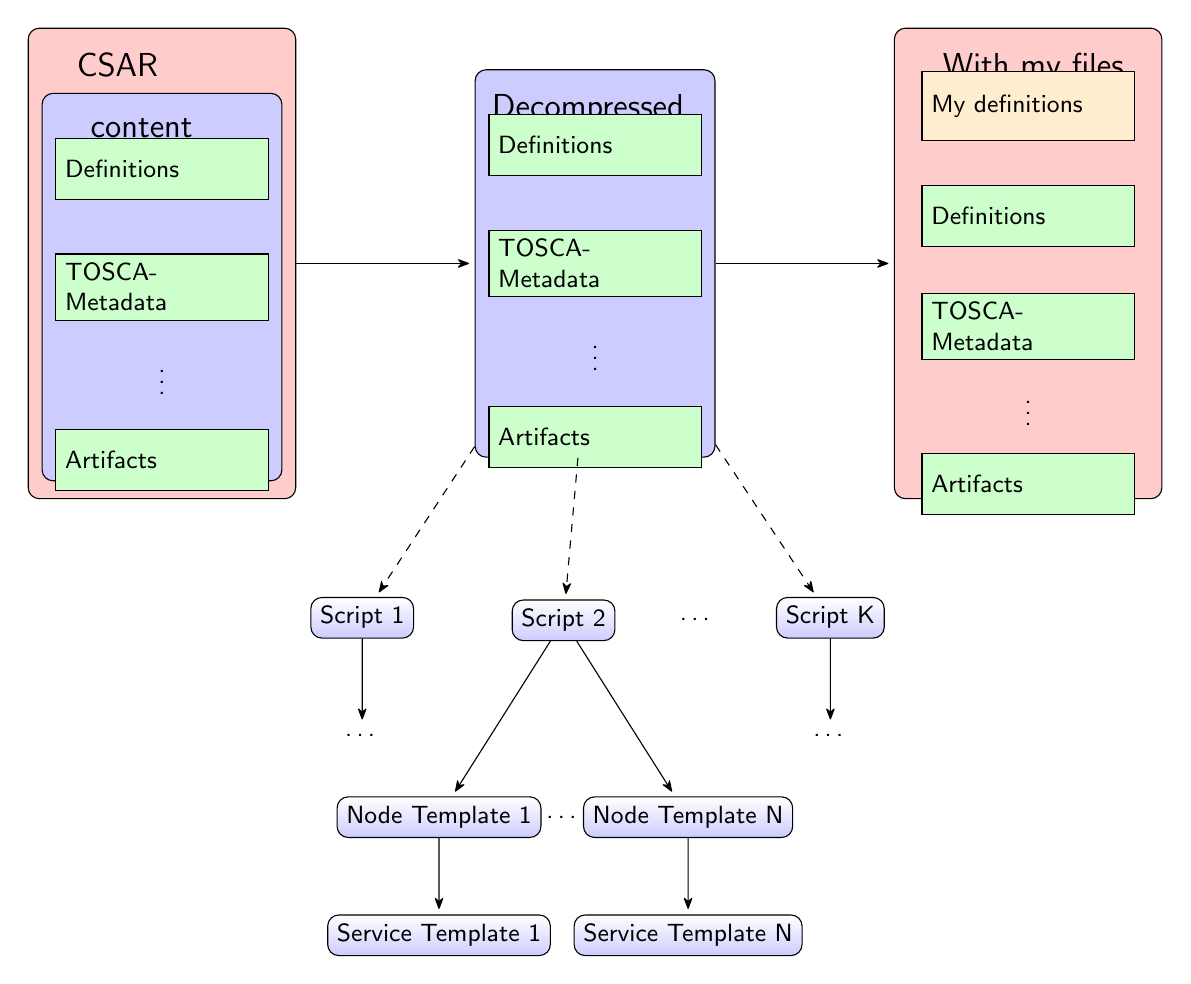
\begin{tikzpicture}[sibling distance=9em,->,>={Stealth[round,sep]},shorten >=1pt,auto,node distance=25mm]


\node (csar_frame) [frame] {};
\node [xshift=+5mm, yshift=-2mm, below right] at (csar_frame.north west) {\large CSAR};

\node (csar_content) at ( [yshift=-3mm]csar_frame) [csar_content] {};
\node [xshift=+5mm, yshift=-2mm, below right] at (csar_content.north west) {\large content};

\node (l2pm1) at ([yshift=+15mm]csar_content) [entry] {Definitions\\};
\node (l2pm2) at ([yshift=0mm]csar_content) [entry] {TOSCA-Metadata\\};
\node (l2pmn) at ([yshift=-22mm]csar_content) [entry] {Artifacts\\};
\node at ($(l2pm2)!.5!(l2pmn)$) {\vdots};
    
\node [right of=csar_frame, xshift=30mm](dc_frame) [csar_content] {};
\node [xshift=+1mm, yshift=-2mm, below right] at (dc_frame.north west) {\large Decompressed};
\draw [->] (csar_frame) -- (dc_frame);
\node (2pm1) at ([yshift=+15mm]dc_frame) [entry] {Definitions\\};
\node (2pm2) at ([yshift=0mm]dc_frame) [entry] {TOSCA-Metadata\\};
\node (2pmn) at ([yshift=-22mm]dc_frame) [entry] {Artifacts\\};
\node at ($(2pm2)!.5!(2pmn)$) {\vdots};

\node [right of=dc_frame, xshift=30mm](my_frame) [frame] {};
\node [xshift=+5mm, yshift=-2mm, below right] at (my_frame.north west) {\large With my files};
\draw [->] (dc_frame) -- (my_frame);
\node (3pmd) at ([yshift=+20mm]my_frame) [myentry] {My definitions\\};
\node (3pm1) at ([yshift=+6mm]my_frame) [entry] {Definitions\\};
\node (3pm2) at ([yshift=-8mm]my_frame) [entry] {TOSCA-Metadata\\};
\node (3pmn) at ([yshift=-28mm]my_frame) [entry] {Artifacts\\};
\node at ($(3pm2)!.5!(3pmn)$) {\vdots};


\node[below=of dc_frame,main node, node distance=10mm, xshift=-4mm, yshift=+7mm] (11) {Script 2}
child { node[main node, yshift=-10mm]  (n21) {Node Template 1} 
		child { node[main node] (s31) {Service Template 1}}  
}
child { node[main node, yshift=-10mm]  (n22) {Node Template N} 
	child { node[main node] (s32) {Service Template N}}  
};
\draw [dashed,->] (dc_frame) -- (11);
\node[below left=of dc_frame,main node,xshift=+10mm] (12) {Script 1}
child { node  {\ldots} 
};
\draw [dashed,->] (dc_frame) -- (12);
\node[below right=of dc_frame,main node, xshift=-10mm] (13) {Script K}
child { node  {\ldots} 
};
\draw [dashed,->] (dc_frame) -- (13);
\node at ($(11)!.5!(13)$) {\ldots};
\node at ($(n21)!.5!(n22)$) {\ldots};

\end{tikzpicture} 
\caption{Preprocessing: decompression, adding files and generating dependencies} 	\label{fig:preproc}
\end{figure}

\subsection{Language Modules} \label{subs:archlm}
Each $language$ $module$ describes a handling of one language and chooses files written in the language.
It also contains a list of supported package manager modules.
Each language module must provide the capability to generate a TOSCA node for the given package and this node must use the same language to install the package.
For example a Bash module must provide capability to define new package nodes which use bash to install the packages.
This means that a script and definitions for Artifact Templates, a Node Type, and a Node Type Implementation should be created by a language module.\\
As it is already mentioned above, during the $processing$ stage a language module analyzes all files one by one and checks their belonging to the language. 
Any files not belonging to the described language are filtered out.
The remaining files are transferred to the language module's $package$ $manager$ $modules$.
For example, a $bash$ module will pass only files with $".sh"$ extension which start with the $"\#!/bin/bash"$ line.
An $ansible$ module should have an additional functionality to unpack zip archives where ansible playbooks can be stored.
Since ansible playbooks don't contain a specific header or marker, the single sign of ansible files is the "$.yml$" extension. 
In the single node mode it will collect names of required packages from the corresponding package manager modules and create a single TOSCA node for all of them.

\subsection{Package Manager Modules} \label{subs:archpmm}
These modules handle different package managers.
They are integrated into language modules and become from them files to analyze.
They must identify package installation commands which use the handled package manager.
In normal mode a $package$ $managers$ $module$ finds external references, resolves them and transmits the package name to the $package$ $handler$ described in the next section.
After transmitting the names to the package handler, it must return the list of all required packages back to the language module to transfer them farther back to a language module.\\
Figure~\ref{fig:lang_ph} illustrates data flow between language modules, package manager modules and the package handler.
To resolve an external reference a package manager module will parse the given file. 
In the case of the apt-get module for bash, the module will read a file line-by-line searching for the commands starting with "apt-get install".
Such commands must be commented out and their arguments should be divided into separate package names which will be transferred to the package handler. 
% !TeX spellcheck = en_US
\usetikzlibrary{calc,arrows.meta,positioning}
\tikzset{
    every node/.style={font=\sffamily\small},
    main node/.style={shape=rectangle, rounded corners,
    	draw, align=center,
    	top color=white, bottom color=blue!20},
    data node/.style={shape=rectangle,
    draw, align=center,
    top color=white, bottom color=red!20}
}

\begin{figure}
	\centering
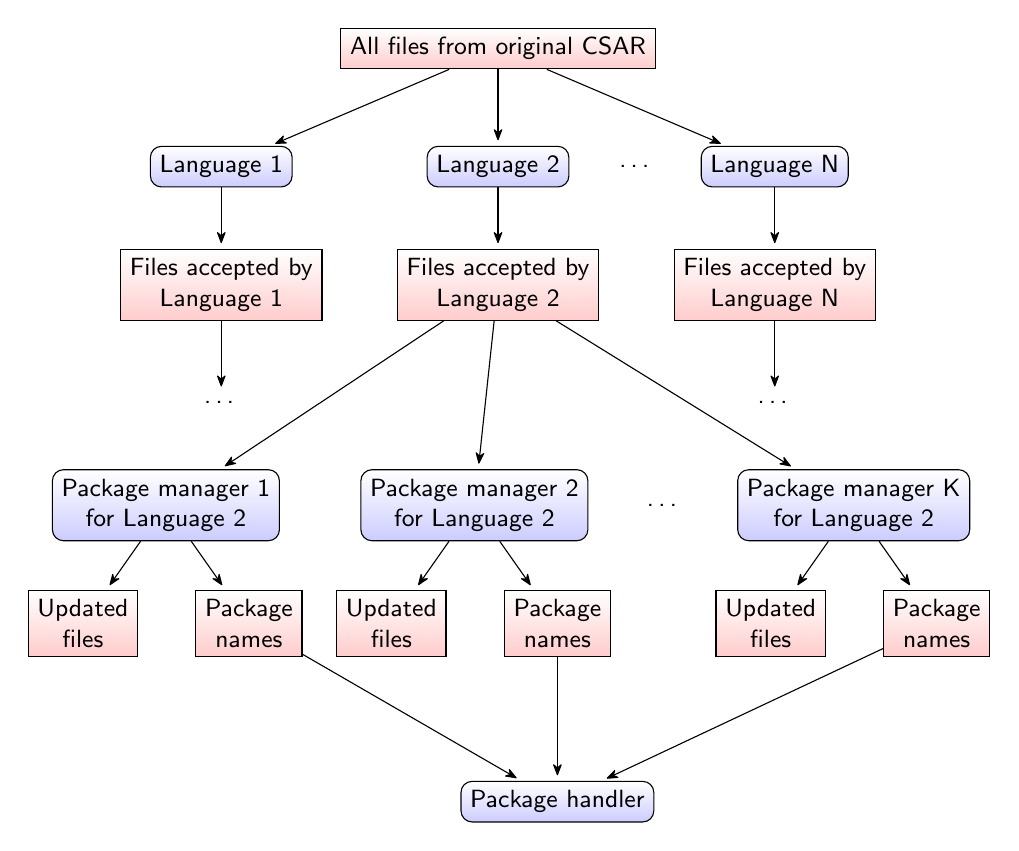
\begin{tikzpicture}[->,>={Stealth[round,sep]},shorten >=1pt,auto,level 1/.style={sibling distance=10em,node distance=25mm},
level 2/.style={sibling distance=8em,node distance=30mm},
level 3/.style={sibling distance=12em,node distance=30mm},
level 4/.style={sibling distance=6em,node distance=25mm},
level 5/.style={sibling distance=8em,node distance=25mm},
level 6/.style={sibling distance=8em,node distance=25mm}]
    \node[data node] (1)  {All files from original CSAR}
    child { node[main node](2) {Language 1} 
    	child { node[data node](21) {Files accepted by\\ Language 1} 
    		child { node {\ldots}}}}
	child { node[main node] (3) {Language 2}
		child { node[data node](31) {Files accepted by\\ Language 2} 
			child { node[main node, yshift=-13mm](32) {Package manager 1\\for Language 2} 
				child { node[data node](36) {Updated\\ files}}
				child { node[data node](37) {Package\\ names}}}
			child { node[main node, yshift=-13mm, xshift=-3mm](33) {Package manager 2\\for Language 2}
				child { node[data node](34) {Updated\\ files}}
				child { node[data node](35) {Package\\ names}}}
			child { node[main node, yshift=-13mm, xshift=+3mm](34) {Package manager K\\for Language 2}
				child { node[data node](38) {Updated\\ files}}
				child { node[data node](39) {Package\\ names}}}
			}
		}
    child { node[main node] (4) {Language N}
    	child { node[data node](41) {Files accepted by\\ Language N} 
    		child { node {\ldots}}}}
	;

	\node [main node,below, yshift=-20mm] at (35) (ph) {Package handler};
    \node at ($(3)!.5!(4)$) {\ldots};
    \node at ($(33)!.5!(34)$) {\ldots};
    \draw [->] (35) --(ph);
    \draw [->] (37) --(ph);
    \draw [->] (39) --(ph);
    
\end{tikzpicture} 
\caption{Data flow scheme between language modules, package manager modules and package handler.} 	\label{fig:lang_ph}
\end{figure}

\subsection{Download Tool Modules}
A download tool module process the defined data download tool.
It analysis the files provided by a language module which it was defined in.
Identified external references must be resolved by removing installation commands, downloading files and transferring them to the topology handler described later.
Behavior features will be defined by the selected operation mode.

\subsection{Package Handler} \label{subs:archph}
The $package$ $handler$ provides interface to communicate with an operating system's package manager. 
It can download installation data, determine the type of dependency between packages and provide a list with dependent packages for a given package.
To download the installation data this component will use given package name and the architecture specified by the CSAR handler.
Then it transfers the package name to the $topology$ $handler$ and repeats the actions for all depended packages recursively. 
In the process it stores all names of packages from the dependency tree of original package and sends them back to the calling package manager module.
To download the data the command "apt-get download \textbf{package}" can be used. 
The architecture can be specified by a ":$architecture$" suffix, for example, a "package:arm" mean the package for the $arm$ architecture.
The list of dependencies will be obtained using the "apt-cache depends \textbf{package}" command. 
The output of such command should be parsed in order to extract names of depended packages.
Type of dependency can be achieved in the same manner.
Of course, in case of a fault during a download of a package, a user interface should be provided to find a solution.
It can be: retry the download, ignore the package, rename the package or even break the framework's execution.

\subsection{Topology Handler} \label{subs:archtop}
%This element should handle the TOSCA topology and it has two main tasks: to analyze the TOSCA topology during the preprocessing stage to create internal dependencies trees and to use those trees to create TOSCA definitions for Node Templates and Relationship Templates in the right places for the packages provided by the package handler.
This element should handle the TOSCA topology and it has two main tasks: create internal dependencies trees and generate TOSCA definitions for packages provided by the package handler.
To build the trees the analysis of the TOSCA topology will be used during the preprocessing stage.
This procedure was described in section~\ref{subs:analyse}.
The needed TOSCA definitions for new package node include Node Templates and Relationship Templates which were described in section~\ref{subs:repres}.
To create the definitions in the right places the generated internal dependencies trees will be used.
The internal dependencies trees must be updated to represent changes after addition of new Node Templates and Relationship Templates.
%$Topology$ $handler$ adds a package to the topology. 
%This includes adding new files and updating existing files. 
%Necessary steps were described in section \ref{subs:repres}.